\documentclass[a4paper,11pt]{article}
\pdfoutput=1 % if your are submitting a pdflatex (i.e. if you have
             % images in pdf, png or jpg format)

\usepackage{jinstpub} % for details on the use of the package, please
                      % see the JINST-author-manual

\usepackage[utf8]{inputenc}           % <- удалить после перевода!!!!!!!!!!!!!!!!!!!!!!!!!!
\usepackage[english, russian]{babel}  % <- удалить после перевода!!!!!!!!!!!!!!!!!!!!!!!!!!


\graphicspath{{figures/}} % Пути к изображениям

\title{\boldmath Investigation of energy spectrum and chemical composition of primary cosmic rays in 1--100 PeV energy range with a drone-borne installation}


% more complex case: 4 authors, 3 institutions, 2 footnotes
\author[a,1]{D.~Chernov,\note{Corresponding author.}}
\author[a]{E.~Bonvech,}
\author[c,d]{M.~Finger~Jr.,}
\author[c,d]{M.~Finger,}
\author[b]{V.~Galkin,}
\author[b]{V.~Ivanov,}
\author[a,b]{D.~Podgrudkov,}
\author[a]{T.~Roganova,}
\author[a,b]{I.~Vaiman}

% The "\note" macro will give a warning: "Ignoring empty anchor..."
% you can safely ignore it.

\affiliation[a]{Lomonosov Moscow State University, Skobeltsyn Institute for Nuclear Physics, Moscow, Russian Federation}
\affiliation[b]{Lomonosov Moscow State University, Faculty of Physics, Moscow, Russian Federation}
\affiliation[c]{Charles University, Faculty of Mathematics and Physics, Prague, Czech Republic}
\affiliation[d]{Joint Institute for Nuclear Research, Dubna, Russian Federation}

% e-mail addresses: only for the corresponding author
\emailAdd{chr@dec1.sinp.msu.ru}


\abstract{This work is dedicated to the development of a project aimed at the implementation of a relatively new method of studying the PCR --- the registration of optical Vavilov-Cherenkov radiation, often called “Cherenkov light”, from EAS (EAS CL), reflected from the snow surface. The objective of the project is to create an installation for the study of the cosmic ray mass composition in the energy range of 1--100 PeV by detecting the reflected EAS CL. Silicon photomultipliers are planned to be used in the detector of the installation, and an unmanned aerial vehicle (UAV, drone) will be used to lift the measuring equipment over the snow-covered surface.}


\keywords{Cherenkov detectors, Mass spectrometers, Balloon instrumentation.}

%\arxivnumber{1234.56789} % only if you have one

% if you write for a special issue this may be useful
\proceeding{Instrumentation for Colliding Beam Physics, INSTR20\\
from 24 to 28 February, 2020\\
Novosibirsk, Russia}



\begin{document}
\maketitle
\flushbottom

\section{Introduction}
\label{sec:intro}

The  1--100 PeV energy range is transitional from galactic to extragalactic cosmic rays. More than 50 years ago a change in the slope of the energy spectrum of primary cosmic rays (PCR) was detected at around 3 PeV. But until now new features in the structure of the spectrum are being discovered. In this regard it is interesting to understand the cause of these slope irregularities. The main reason, most likely, are changes in the mass composition of the PCR. Presently used methods allow to estimate either the average mass of PCR particles or to divide them into ``light''' and ``heavy'' groups. Basically, estimates are made on the reconstructed depth of development maximum of the extensive air showers (EAS), using the the modelling of the shower development in the atmosphere. Since the methodological uncertainties of the reconstructed parameters mass groups can be identified only by processing a large amount of experimental data.

The project is aimed at development of a unique detector using modern photodetectors based on silicon photomultipliers (SiPM), which is installed on an unmanned aerial vehicle. Currently, there are no other devices and installations that would successfully use reflected Cherenkov light registration method. The method allows to achieve the highest accuracy of estimation of the chemical composition of PCR in the analysis of the individual EAS events in comparison with existing ground installations. The successful implementation of the project will allow obtaining experimental data for the reconstruction of partial spectra for several mass groups of PCR particles (protons, helium, CNO and Fe groups) in the 1--100 PeV energy range.


\begin{figure}[t]
\centering
\includegraphics[height=.4\textheight]{Sphere2Baikal.png}
\caption{\label{fig:Sphere_Baikal} Experiment with the SPHERE-2 installation on lake Baikal.}
\end{figure}


\section{Registration methods}
\subsection{Method overview}
We propose to apply a reflected Cherenkov light registration method~\cite{}(\textbf{ссылка на описание метода!!!}) for this experiment. The main idea of this method consists in the detection of the extensive air showers Cherenkov light reflected from the snowed earth surface using the compact apparatus lifted above ground. The initial idea was first introduced by A.E. Chedakov in~\cite{} (\textbf{ссылка на Чудакова}). Later the technique was successfully used in our earlier experiments~\cite{1,2}.

The proposed method has a number of advantages over traditional EAS registration methods. They are as follows:
\begin{itemize}
\item Provides a significant area of CL registration using a compact device;
\item Accurate estimation of PCR energy in an individual event in comparison with other methods;
\item The field of view of the individual sensitive elements of the device covers a significant part of the surveyed area, which allows observation the CL from EAS near the shower axis, usually inaccessible to ground-based CL detector arrays. This circumstance significantly increases the accuracy of the primary particle type estimation;
\item Allows measurement of the same PCR energy range with different resolution (distance between the centres of the fields of view of neighbouring sensing elements) using variation of the detector elevation, which allows you to control the magnitude of systematic errors.
\end{itemize}

\subsection{Previous detector realizations}
In the period from 2008 to 2013, a series of measurements of reflected Cherenkov light was carried out using the SPHERE-2~\cite{1,2,3} balloon detector. Measurements were made under the snow-covered ice of Baikal lake. The Figure~\ref{fig:1} shows the landing point on the Baikal lake surface and the special BAPA balloon designed for the experiment. 

The SPHERE-2 apparatus was constructed with a 1.5~m diameter spherical mirror with the 93 cm Shmidt diaphragm window. Cherenkov light was detected by 109 PMT retina located near the focus of the spherical mirror. The scheme of the optical part of the detector is shown in the box on the Figure~\ref{fig:Sphere_Baikal}.

The energy spectrum of all particles was measured. And the light nuclei part estimation~\ref{fig:Sphere_results} was calculated. The results was published in~\cite{2}. 

\begin{figure}[t]
\centering % \begin{center}/\end{center} takes some additional vertical space
\includegraphics[width=.4\textwidth]{sphere2spectrum.png}
\qquad
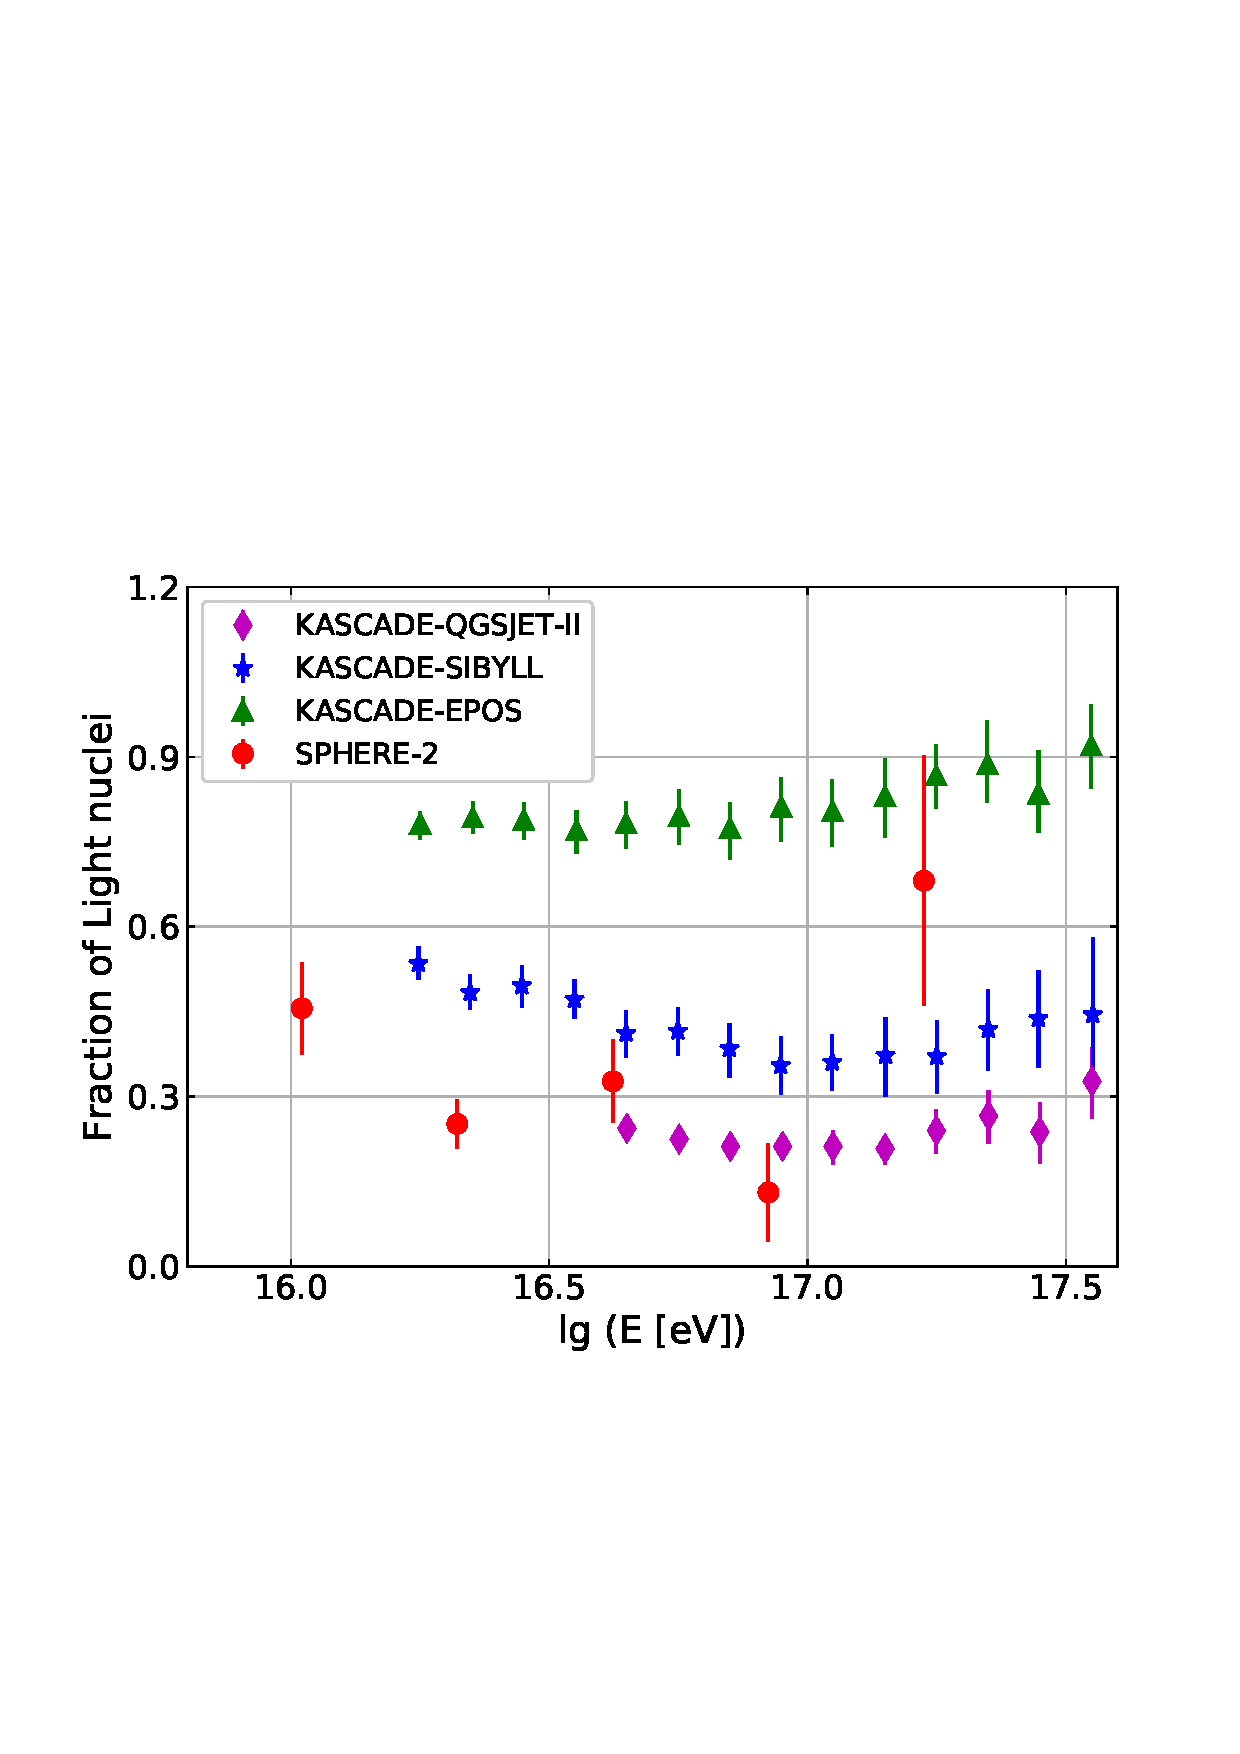
\includegraphics[width=.4\textwidth]{sphere2composition.png}
% "\includegraphics" from the "graphicx" permits to crop (trim+clip)
% and rotate (angle) and image (and much more)
\caption{\label{fig:Sphere_results} Results of the SPHERE-2 experiment. Energy spectrum (left) and chemical composition estimates (right).}
\end{figure}

The SPHERE-2 apparatus hadn't fully utilized all the possibilities of the method. %The main problem of the measurements with the SPHERE-2 was a small number of recorded events, and, therefore, insufficient statistical reliability of the results on the chemical composition. 
This was due to two main reasons.

The first reason is the low sensitivity of the matrix used by the PMT.

The small sensitive area and low quantum efficiency of the FEU-84 PMT, used in the detector, reduced the expected statistical material by more than 5 times due to the increase in the energy threshold of registration.

The second reason was the technical difficulties associated with the need to maintain the balloon in working condition for the multiple launches of the detector.

Each 10-day measurement session required at least 6 tons of cargo with helium cylinders to be transported to the measurement site, so no more than one session was possible per year.

While in winter it is possible to hold up to 5 sessions per year.

Taking into account all the above difficulties we have developed a new detector based on SiPM Cherenkov light sensor.
Small mass of the detector will allow to abandon the cumbersome and time-consuming in use balloon and switch to the UAVs (drones) as a carrier.
This experimental setup has never been used before in the study of ultra high energy PCR.
Currently, in the field of ultrahigh energy cosmic rays astrophysics, UAVs are used only for solving auxiliary tasks as monitoring the atmosphere and calibrating ground detectors.


\section{The detector}

The group of this project obtained unique results using this new technique (see section 2). 
Good methodological accuracy of the measurements opens up good prospects for the development of projects for new experiments. 

Based on the operating experience of the SPHERE-2 detector, it is possible to develop detectors superior in their capabilities to many ground installations.

Advantages of the described technique and progress in the field of microelectronics already allows design of the compact detector of the reflected CL from EAS with big effective area of registration, a wide viewing angle (for PCR) and high spatial resolution. 

Indeed, comparing a ground detector arrays with an effective area of about 1 km$^2$ and more, service
infrastructure, etc., and a compact detector weighing up to 10 kg with similar characteristics (geometric factor), the differences in the amount of material and labor costs to obtain comparable scientific results become obvious. 

For an installation with a large registration area, the costs can vary by tens or even hundreds of times.



It is planned to design a compact detector that will have the following characteristics:

\begin{itemize}
\item Sensitive area of optics (aperture input window) around 0,1m$^2$;
\item Mirror diameter 80 or 100 cm;
\item Optical system viewing angle up to $\pm$25 degrees;
\item Number of mosaic elements 133--259 SiPM;
\item The mass of the detector less 10 kg;
\item The flight height of the detector 300--700~m;
\item Expected number of events EAS (with $E_0$ = 1--100 PeV) up to 3\,000 for season.
\end{itemize}

\begin{figure}[bt]
\centering % \begin{center}/\end{center} takes some additional vertical space
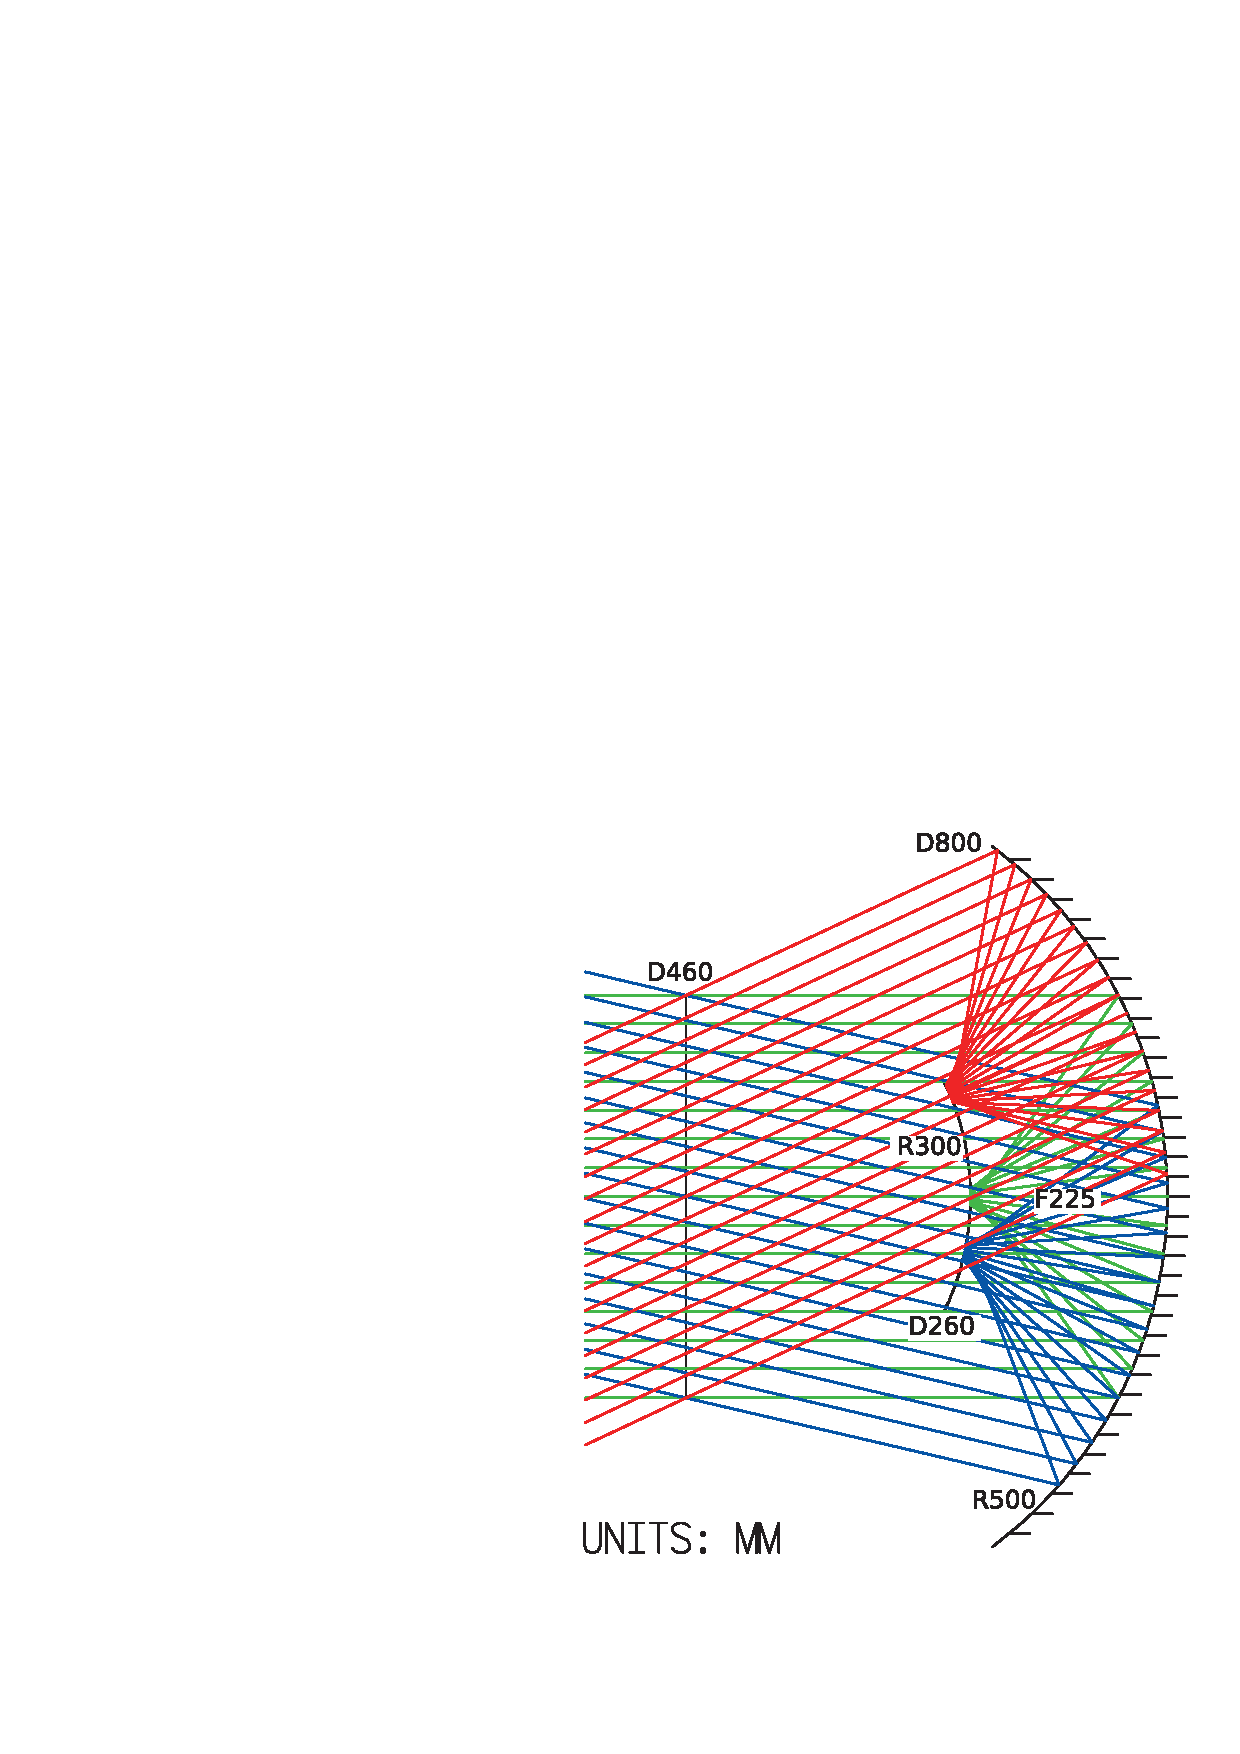
\includegraphics[width=.32\textwidth,clip]{Sphere3optic.png}
\qquad
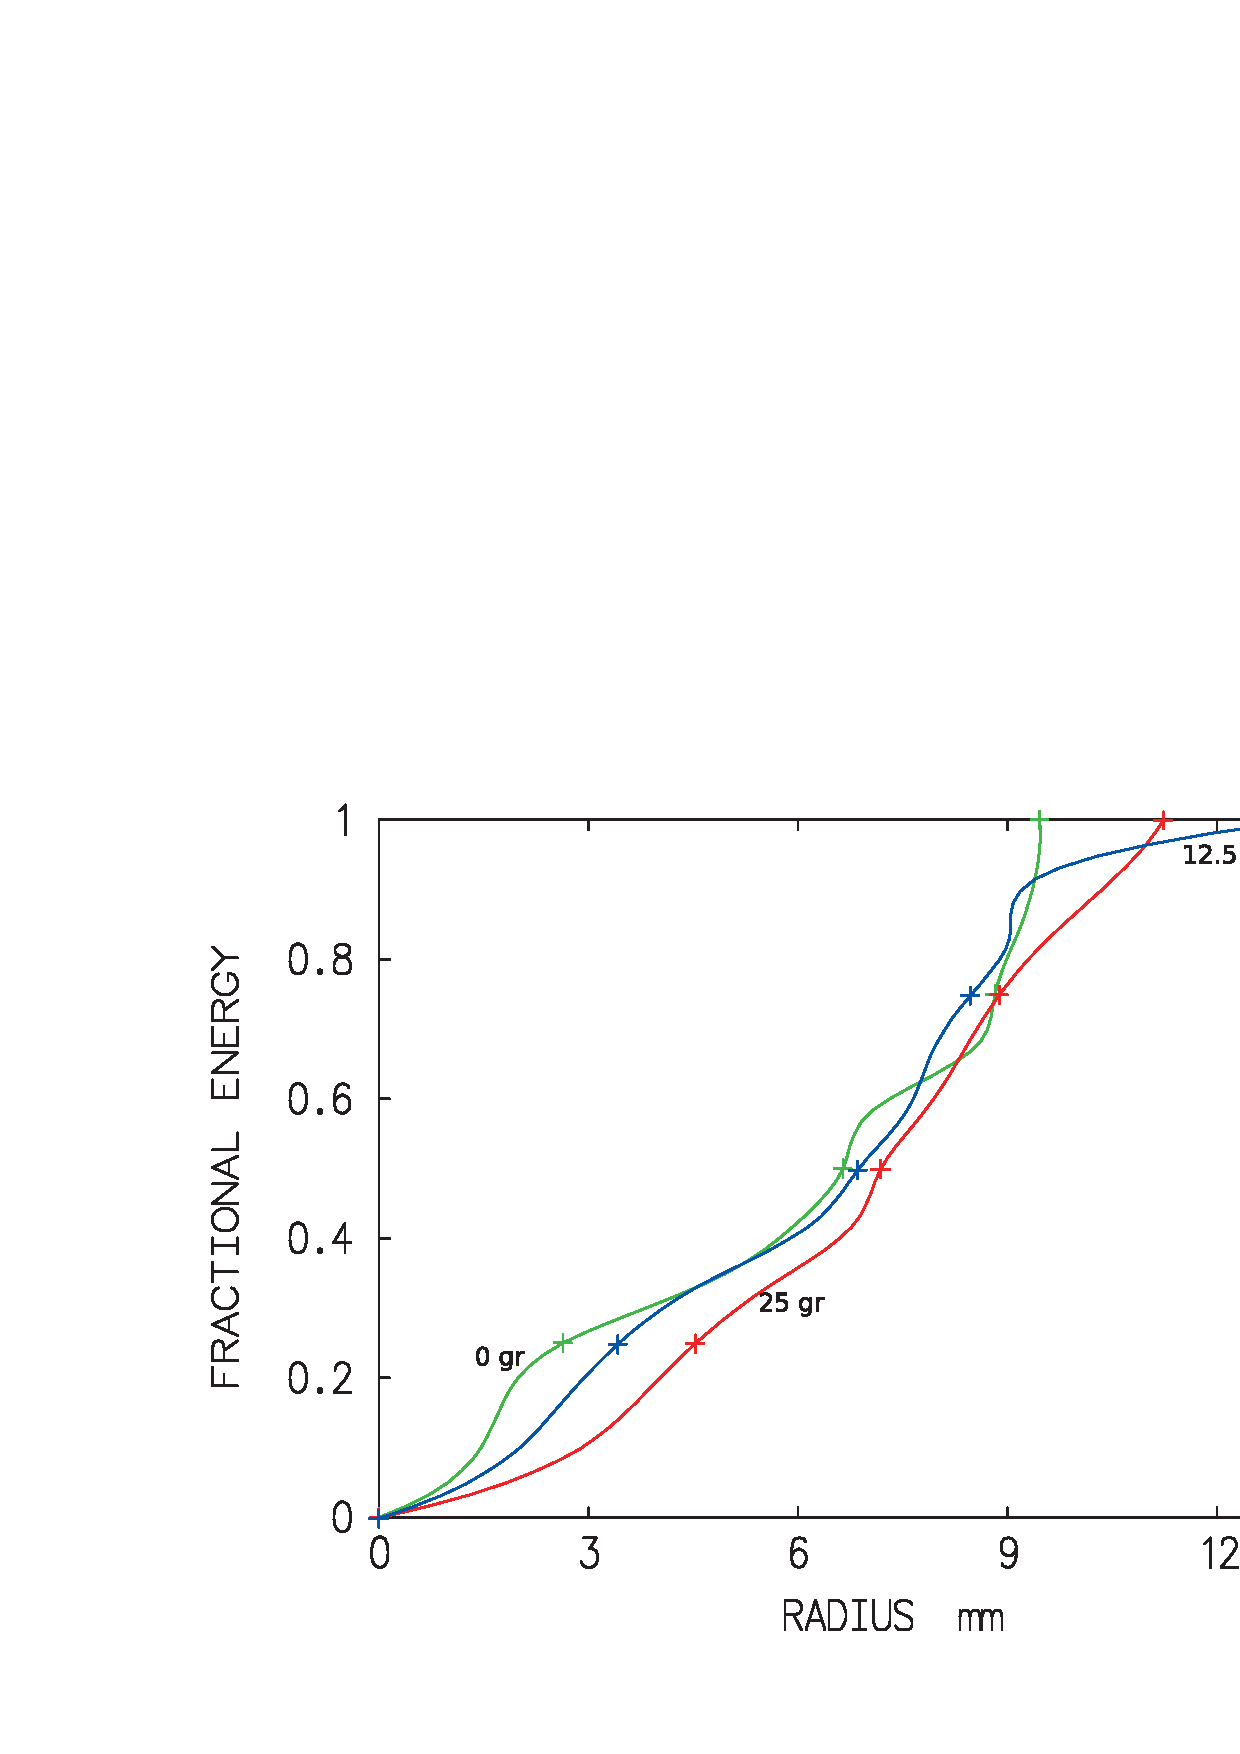
\includegraphics[width=.48\textwidth]{Sphere3spot_energy.png}
\caption{Optical scheme of the developed detector (without shadow of the mosaic) and the fractional light energy distribution on focal plane taking into account the shadow from the mosaic. Red color corresponds to the rays coming at an angle of 25$^\circ$ from the optical axis, blue --- 12.5$^\circ$ and green --- paraxial.}
\label{fig:optic_sphere3}
\end{figure}

One of the optical scheme variants based on the simplified Schmidt scheme (no corrector plate) is shown in the figure~\ref{fig:optic_sphere3} (left). The rays are shown without the absorption on the backside of the SiPM mosaic for illustration only. The detector is planned to have a spherical 800~mm diameter mirror with 500~mm curvature radius. The 460~mm diameter diaphragm situated 550~mm from the mirror.

The image of the reflected shower is formed on the photosensitive spherical surface with 260~mm diameter and 300~mm curvature radius. The optimum distance for this set of parameters is 225~mm from the mirror. Maximum observation angle is 25$^\circ$.

On the figure~\ref{fig:optic_sphere3} (right) the relative amount of light collected within the certain radius is shown. Different colors shows different incidence angle relative to the detector optical axis.

On the figure~\ref{fig:spots} the light spots on the photosensitive detector surface are show for different conditions - three light incidence angles on the detector (0$^\circ$, 18$^\circ$ and 25$^\circ$) and five offsets of the photosensitive surface. For the reference a 20~mm scale line is shown in the lower left corner. The spots were calculated for the 420~nm wavelength.

\begin{figure}[bt]
\centering
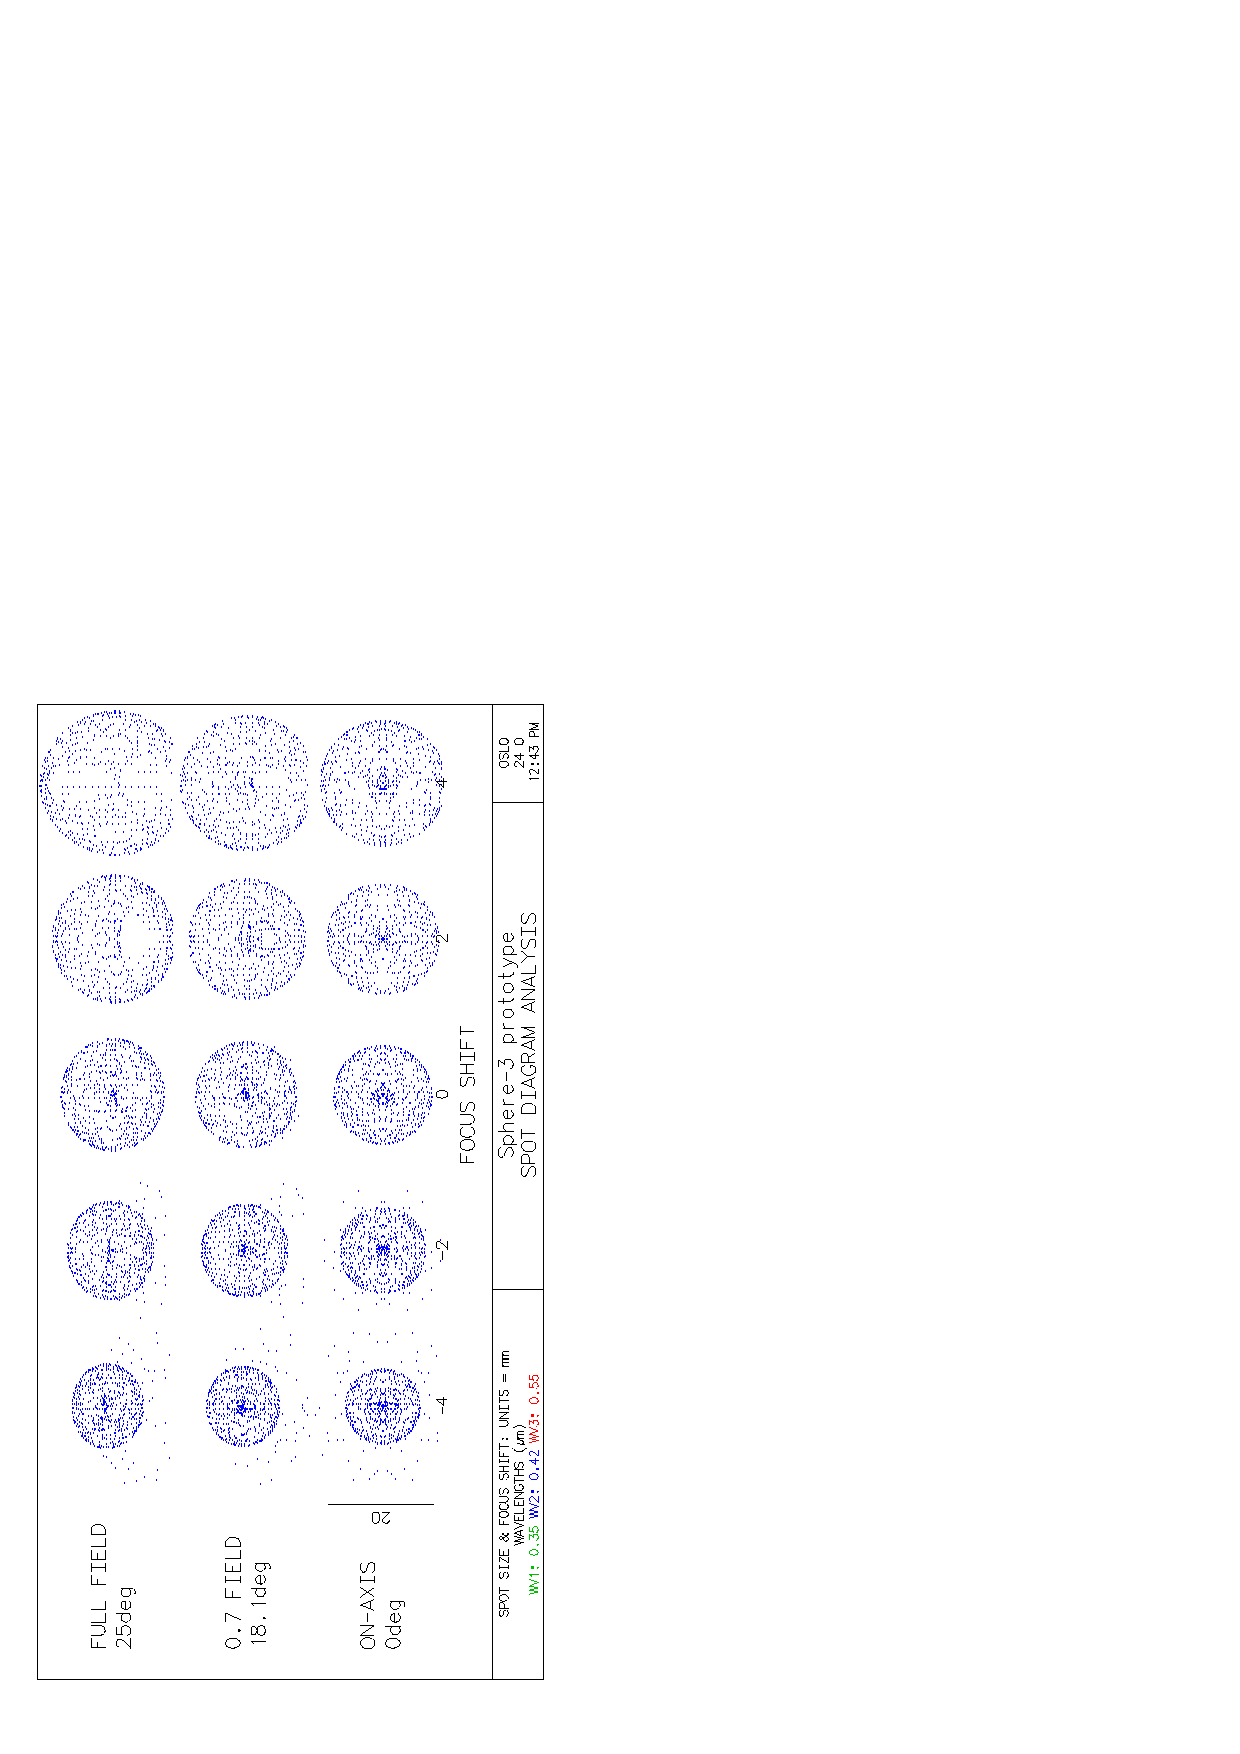
\includegraphics[width=.8\textwidth]{Sphere3spot.png}
\caption{ Images of light spots on the focal surface of the detector from point light sources taking taking into account the shadow from the mosaic. All values in mm}
\label{fig:spots}
\end{figure}    

The mirror for the detector will be made on the basis of composite materials. The mirror base is made of cellular aluminium This design has sufficient rigidity and low weight.

\begin{figure}[t]
\centering % \begin{center}/\end{center} takes some additional vertical space
\includegraphics[width=.55\textwidth]{mosaic_protype.png}
\caption{The matrix prototype of 49 SiPM is assembled from seven electronic boards of 7 SiPM with preamps.}
\label{fig:mosaic49_7}
\end{figure}

The main element of the new installation will be a segment of seven SiPM Micro FC-60035 SiPMs. The tests of a matrix of seven such segments (49 SiPM) was successfully completed (see figure~\ref{fig:mosaic49_7}). Each segment was equipped with seven preamplifiers and a temperature sensor to account for the effects of thermal emission. Each SiPM was equipped with a light collector CA10929 Boom-MC-W with angular characteristic $\pm$24 degrees at 50\% effectiveness. In this project, it is planned to modify and adapt the SiPM segment for use in a ultra-wide angle optical system.

To register analogue signals from SiPMs, a digitization board based on the ADS5296A 8-channel fast analog-to-digital converter (FADC) chip will be developed.
The measurement period of this chip is up to 12.5 ns at 12-bit resolution and 10 ns at 10-bit resolution.
The board design allows to reduce time of digitization by a factor of 2 by installing two FADC on each SiPM.
Small size of the chip (9x9 mm) allows significant reduction of the detector weight and dimensions. 
Digitized signals from each channel in serial code are transmitted to the LVDS interface on the PicoZed - XC7Z030-1SBG485 module with a programmable logic chip.
These chips are equipped with a built-in computer running the Linux operating system.
All internal logic of the measuring system and the trigger system is recorded in the chip as a configuration file in accordance with the program in the VHDL language of integrated circuit equipment description.
The measurement results are recorded on the micro-SD memory card of the built-in computer for further processing.


\section{Hardware and calculation development plan}

Stages of experiment:
\begin{enumerate}
\item Generation of images of artificial EAS events in the detector mosaic and analysis of spacial-temporal and spacial-angular distributions of Cherenkov light for the purpose of finding optimal criteria for the selection of genuine EAS events and separation of showers according to the mass of primary particles.
\item Modification of the design of the apparatus in accordance with the results of the 1st stage.
\item Development of the data processing algorithms appropriate to the hardware properties.
\item Ground tests.
\item Actual measurements.
\item Data processing with the criteria previously developed, improvement of the criteria and data re-processing.
\end{enumerate}


\begin{figure}[t]
\centering % \begin{center}/\end{center} takes some additional vertical space
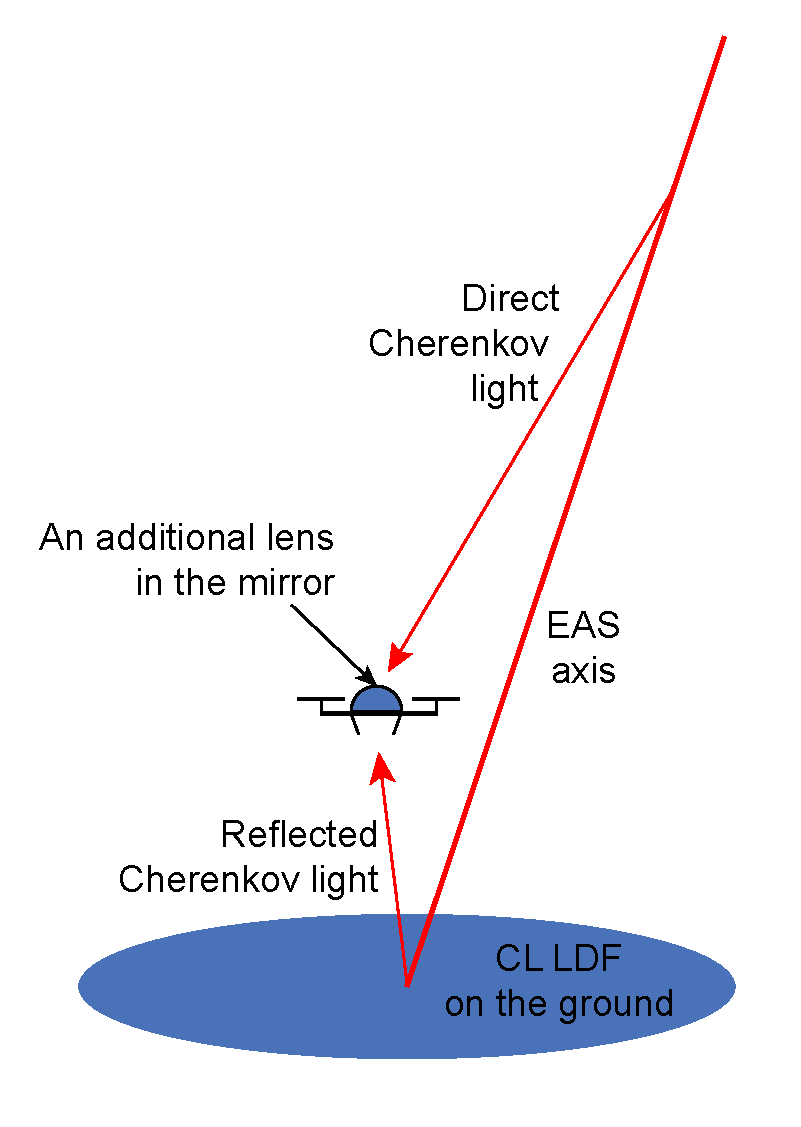
\includegraphics[width=.35\textwidth]{DirectCL.png}
\caption{\label{fig:DirectCL} Scheme of direct and reflected Cherenkov light of EAS.}
\end{figure}

The detector will use the simplified Schmidt optical system. In this system, the central part of the mirror is not used since it is in the shadow of the photodetector. A hole in the centre of the mirror with a wide-angle lens in it with an aperture of about 100 cm$^2$ will allow registration of the direct CL (see figure~\ref{fig:DirectCL}). Calculations show that for EAS from PCR with 1 PeV energy the CL photons density is around 100 photons per cm$^2$ at a distance of 100 m from the shower axis. Taking into account the SiPM quantum efficiency and losses of optical elements expects to register around 1000 photoelectrons.
%The estimation of the primary particle mass can use the information on the intensity of the direct CL in addition to the data on the reflected CL.

  The main function of the direct CL detection is to increase both the sensitivity and the specificity of the criterion separating actual EAS events using the correlated signals of direct and reflected CL. It is already clear that accurate detection and analysis of CL angular distribution can yield substantial information on the PCR mass composition~\cite{5,6}  but such an experiment requires a large and more complex detector or even an array of such detectors placed wide apart, e.g. borne by a few drones.

  Still, one can say the second function of the direct CL detection channel is a preliminary study of the possibility to estimate the shape and angular size of CL flash, which will help us to elaborate a new version of the detector capable of distinguishing between different primary masses using both lateral and angular CL characteristics.

  For the moment the main means of primary mass separation are the criteria based on the shape of EAS CL lateral distribution over the snowed surface seen by SPHERE-3 optical system. Presumably such criteria will work better than with SPHERE-2 due to higher spacial resolution of the new detector.

Primary mass estimation is by far the most difficult part of the primary particle parameter evaluation problem. It is no wonder the PCR mass composition is still poorly known after more than half a century studies. Modeling of EAS CL characteritics~\cite{5,6,7,8}
enables us to put forward some basic principles for choosing the criterial parameters for the primary mass separation:

- such parameter should be directly measurable or, at least, directly calculable from the measured quantities; this property may be called {\it observability};

- another property is called {\it integrality}: the parameter must rely on the substantial part of the whole distribution measured (e.g., appreciable part of CL photons seen by detector); the property ensures the suppression of fluctuations which hinder the process of classification/separation;

- one more important property of a criterial parameter is its {\it relativity}: it must reflect the shape of the distribution of the characteristic measured; this quality makes the parameter weakly dependent on the primary energy and, which is even more important, on the nuclear interaction model at super high energies; the latter feature has already been checked on EAS CL angular and lateral distributions~\cite{5,6,7,8} but will likely hold on other shower characteristic distributions.

After all these points are taken into account one should optimize the definition of criterial parameter with respect to fluctuations. In other words, parameter values must have minimum possible variation for a given primary mass.

%It is assumed that the EAS from the primary proton should form a light spot different of Fe nuclei at the same primary energy and depth of EAS maximum.


\section{The conditions for conducting measurements on a UAV}

During implementation of the project, it is planned to develop a more advanced device with improved spatial resolution and greater aperture. 
In addition, it is possible to use a grouping of several UAVs to proportionally increase the geometric factor and statistical reliability of the results. 
The use of hydrogen-air fuel cells or gasoline drones with a continuous operation time of up to several hours will greatly simplify the measurement process and improve the efficiency of experimental data collection.

To control the density and transparency of the atmosphere an auxiliary small UAV can be used with pressure, temperature, humidity sensors and laser lidar. The lidar will be used to control the reflection from the snow. Laser control of the atmosphere and reflection from the snow will improve the accuracy of measuring the EAS CL.

The properties of the snow surface play an important role when using the method of reflected CL registration. The results of the show optical properties studies have been repeatedly published by several groups. The simulation results show that in the wavelength range from 300 to 600 nm, the relative reflectance for pure snow is stable within 3\% for the zenith angles of the light incidence from 0 to 80 degrees. From the above mentioned results and the known CL spectral characteristics it can be concluded that the snow surface reflects the CL with minor spectral distortions in the range of zenith angles up to 80 degrees and can be used as a screen for the CL registration.



%\acknowledgments

%This is the most common positions for acknowledgments. A macro is
%available to maintain the same layout and spelling of the heading.

%\paragraph{Note added.} This is also a good position for notes added after the paper has been written.


% We suggest to always provide author, title and journal data:
% in short all the informations that clearly identify a document.

\begin{thebibliography}{99}

\bibitem{1}
D. V. Chernov, R. A. Antonov, T. V. Aulova, E. A. Bonvech, V. I. Galkin, T. A. Dzhatdoev, D. A. Podgrudkov, and T. M. Roganova, \textit{Detection of reflected Cherenkov light from extensive air showers in the SPHERE experiment as a method of studying superhigh energy cosmic rays}, \textit{Physics of Particles and Nuclei} {\bf vol} 46, no. 1, 2015, pp. 60–93.

\bibitem{2}
R. A. Antonov, T. V. Aulova, E. A. Bonvech, D. V. Chernov, T. A. Dzhatdoev, M. Finger, V. I. Galkin, D. A. Podgrudkov, and T. M. Roganova, \textit{Event-by-event study of cr composition with the sphere experiment using the 2013 data}, \textit{Journal of Physics: Conference Series} {\bf vol} 632, no. 012090, 2015, pp. 1–8.

\bibitem{3}
R. A. Antonov, E. A. Bonvech, D. V. Chernov, T. A. Dzhatdoev, V. I. Galkin, D. A. Podgrudkov, and T. M. Roganova, \textit{Spatial and temporal structure of EAS reflected Cherenkov light signal}, \textit{Astroparticle Physics} {\bf vol} 108, 2019, pp. 24–39.

\bibitem{4}
R. A. Antonov, E. A. Bonvech, D. V. Chernov, T. A. Dzhatdoev, V. I. Galkin, M. Finger Jr., M. Finger, D. A. Podgrudkov, T. M. Roganova,  A. V. Shirokov, and I. A. Vaiman, 
\textit{The SPHERE-2 detector for observation of extensive air showers in 1 PeV – 1 EeV energy range}, \textit{Astroparticle Physics},
doi: 10.1016/j.astropartphys.2020.102460.

\bibitem{5}
V. Galkin, A. Borisov, R. Bakhromzod, V. Batraev, S. Latipova, A. Muqumov
\textit{A Method for Estimation of the Parameters of the Primary Particle of an Extensive Air Shower by a High-Altitude Detector}
\textit{Moscow University Physics Bulletin} 2018. {\bf 73}. N 2. P. 179 \\
 DOI: 10.3103/S0027134918020078

\bibitem{6}  
Batraev V. V., Galkin V.I. \\
\textit{The separation of air showers by the masses of the primary particles on the basis of the
measured angular distributions of Cherenkov light at mountain level}
\textit{Memoirs of the Faculty of Physics, Lomonosov Moscow State University} 2018. N 3. p. 1830202 (in Russian)

\bibitem{7}  
Antonov R.A., Anohina A.M., Bonvech E.A., Chernov D.V., Dzhatdoev T.A., Galkin V.I., Kirillov A.A., Roganova T.M. \\
\textit{A method for primary proton spectrum measurement at Eo >= 10 PeV with SPHERE-2 telescope}
\textit{Proc. 31 ICRC}, Lodz 2009, v.4, id.434

\bibitem{8}  
Anokhina A.M., Antonov R.A., Bonvech E.A., Galkin V.I., Dzhatdoev T.A., Kirillov A.A., Roganova T.M., Chernov D.V., Shaulov S.B. \\
\textit{Method for measuring the PCR proton spectrum in the energy range of > $10^{16}$ eV} 
\textit{Bulletin of the Lebedev Physics Institute} 2009. v.36, N5, pp. 146-149  

% Please avoid comments such as "For a review'', "For some examples",
% "and references therein" or move them in the text. In general,
% please leave only references in the bibliography and move all
% accessory text in footnotes.

% Also, please have only one work for each \bibitem.


\end{thebibliography}
\end{document}